\documentclass[10pt]{article}

\usepackage[margin=0.82in]{geometry}
\usepackage{amsmath,amssymb}
\usepackage{booktabs}
\usepackage{graphicx}
\usepackage{subcaption}
\usepackage{hyperref}
\usepackage{xcolor}

\setlength{\textfloatsep}{8pt plus 2pt minus 2pt}
\setlength{\floatsep}{8pt plus 2pt minus 2pt}
\setlength{\intextsep}{8pt plus 2pt minus 2pt}

\hypersetup{
  colorlinks=true,
  linkcolor=blue!55!black,
  citecolor=blue!55!black,
  urlcolor=blue!55!black
}

\title{\textbf{Absorption Time and Initial Wealth Dispersion in a Multi-Gambler Ruin Process}}
\author{Gambler's Ruin Experiments}
\date{\today}

\begin{document}
\maketitle

\begin{abstract}
We study a simple multi-player gambler's ruin process in which an even number of gamblers are paired each round and each active pair transfers one dollar by a fair coin flip. The winner is eventually the unique surviving gambler, but the time to absorption can be long and highly variable. The central empirical question is whether absorption time is explained by the initial distribution of wealth. We test the hypothesis that, for fixed total wealth $S$ and number of gamblers $N$, absorption time is increasing in the initial dispersion measure
\[
  \sum_{i<j} A_i A_j
  =
  \frac{S^2}{2}\left(1-\mathrm{HHI}\right),
\]
where $\mathrm{HHI}=\sum_i (A_i/S)^2$. In a small-system sweep with $N=6$, $S=80$, 33 initial wealth vectors, and 50 simulations per vector under each of two pairing policies, the normalized median absorption time is strongly aligned with $1-\mathrm{HHI}$, with $R^2 \approx 0.77$ for both random pairing and ranked-after-warmup pairing. The experiment supports a simple thesis: fair play fixes winner probabilities, but the initial concentration of wealth largely controls the time scale on which monopoly occurs.
\end{abstract}

\section{Premise}

Consider $N$ gamblers, where $N$ is even. Gambler $i$ begins with integer wealth $A_i\geq 0$, and total wealth is conserved:
\[
  S = \sum_{i=1}^N A_i.
\]
At each round, active gamblers are paired. Within each pair, a fair coin decides which gambler receives one dollar from the other. A gambler with zero wealth is inactive. The process ends at the absorption time
\[
  T = \inf\{t: \text{only one gambler has positive wealth at round } t\}.
\]

The eventual winner probability is not the main mystery. Under fair play, wealth is a martingale, and the probability that gambler $i$ eventually owns all wealth is
\[
  \mathbb{P}(i \text{ wins}) = \frac{A_i}{S}.
\]
Thus the initially richest gambler wins most often, but not deterministically.

The more interesting object is $T$. Even when winner probabilities are simple, the time to absorption is noisy, strategy-dependent, and sensitive to the initial wealth profile.

\section{A First Theory of Absorption Time}

For two gamblers with wealths $a$ and $S-a$, the classical fair gambler's ruin result gives
\[
  \mathbb{E}[T] = a(S-a).
\]
This expression is exactly the pairwise product of the two initial stacks. The natural multi-player analogue is therefore
\[
  P(A) = \sum_{i<j} A_i A_j.
\]
This quantity is large when wealth is spread across many players and small when one player already dominates.

The same predictor can be written in concentration form. Let
\[
  p_i = \frac{A_i}{S},
  \qquad
  \mathrm{HHI} = \sum_i p_i^2.
\]
Then
\[
  \sum_{i<j} A_i A_j
  =
  \frac{1}{2}\left(S^2-\sum_i A_i^2\right)
  =
  \frac{S^2}{2}\left(1-\mathrm{HHI}\right).
\]
For fixed $S$, the pairwise-product predictor and $1-\mathrm{HHI}$ are equivalent. This suggests the empirical model
\[
  \frac{T}{S^2}
  \approx
  \alpha + \beta(1-\mathrm{HHI}) + \varepsilon,
\]
or, in unnormalized form,
\[
  T \approx C(N,\pi)\sum_{i<j} A_iA_j,
\]
where $\pi$ denotes the pairing policy.

\section{Pairing Policies}

We compare two policies.

\paragraph{Random pairing.}
Each round, active gamblers are shuffled uniformly and paired in that order. If the number of active gamblers is odd, one gambler sits out.

\paragraph{Ranked-after-warmup pairing.}
For the first $W=3$ rounds, pairing is random. Thereafter, active gamblers are sorted by current wealth and paired by adjacent rank:
\[
  1\text{ vs }2,\quad 3\text{ vs }4,\quad 5\text{ vs }6,\ldots
\]
The individual games remain fair. This policy changes only the interaction graph. Rich gamblers are forced to contest other rich gamblers, while poor gamblers tend to play near peers.

\section{Experimental Design}

We ran a small-system absorption sweep:
\[
  N=6,\qquad S=80.
\]
We generated 33 initial wealth vectors from six distribution families: equal, linear descending, geometric descending, one-whale, two-whale, and Dirichlet-style random splits. For each initial vector and each pairing policy, we ran 50 independent simulations to true absorption. This gives
\[
  33 \times 50 = 1650
\]
simulations per strategy, and 3300 total simulations.

For every initial vector we recorded:
\[
  \mathrm{HHI},\quad
  1-\mathrm{HHI},\quad
  \sum_{i<j}A_iA_j,\quad
  \mathrm{Gini},\quad
  \max_i A_i/S,\quad
  \text{entropy}.
\]
For each vector-strategy pair we summarized the absorption-time distribution by its mean, median, 90th percentile, and 99th percentile. The main response variable below is the normalized median absorption time $T_{\mathrm{med}}/S^2$, which is less tail-sensitive than the mean.

\section{Results}

\subsection{Dispersion predicts absorption time}

Figure~\ref{fig:concentration} plots normalized median and mean absorption time against $1-\mathrm{HHI}$. The relationship is visibly positive: more initially dispersed wealth produces longer time to monopoly. A linear fit using $1-\mathrm{HHI}$ explains roughly 77\% of the cross-vector variation in normalized median absorption time for both strategies.

\begin{figure}[htbp]
  \centering
  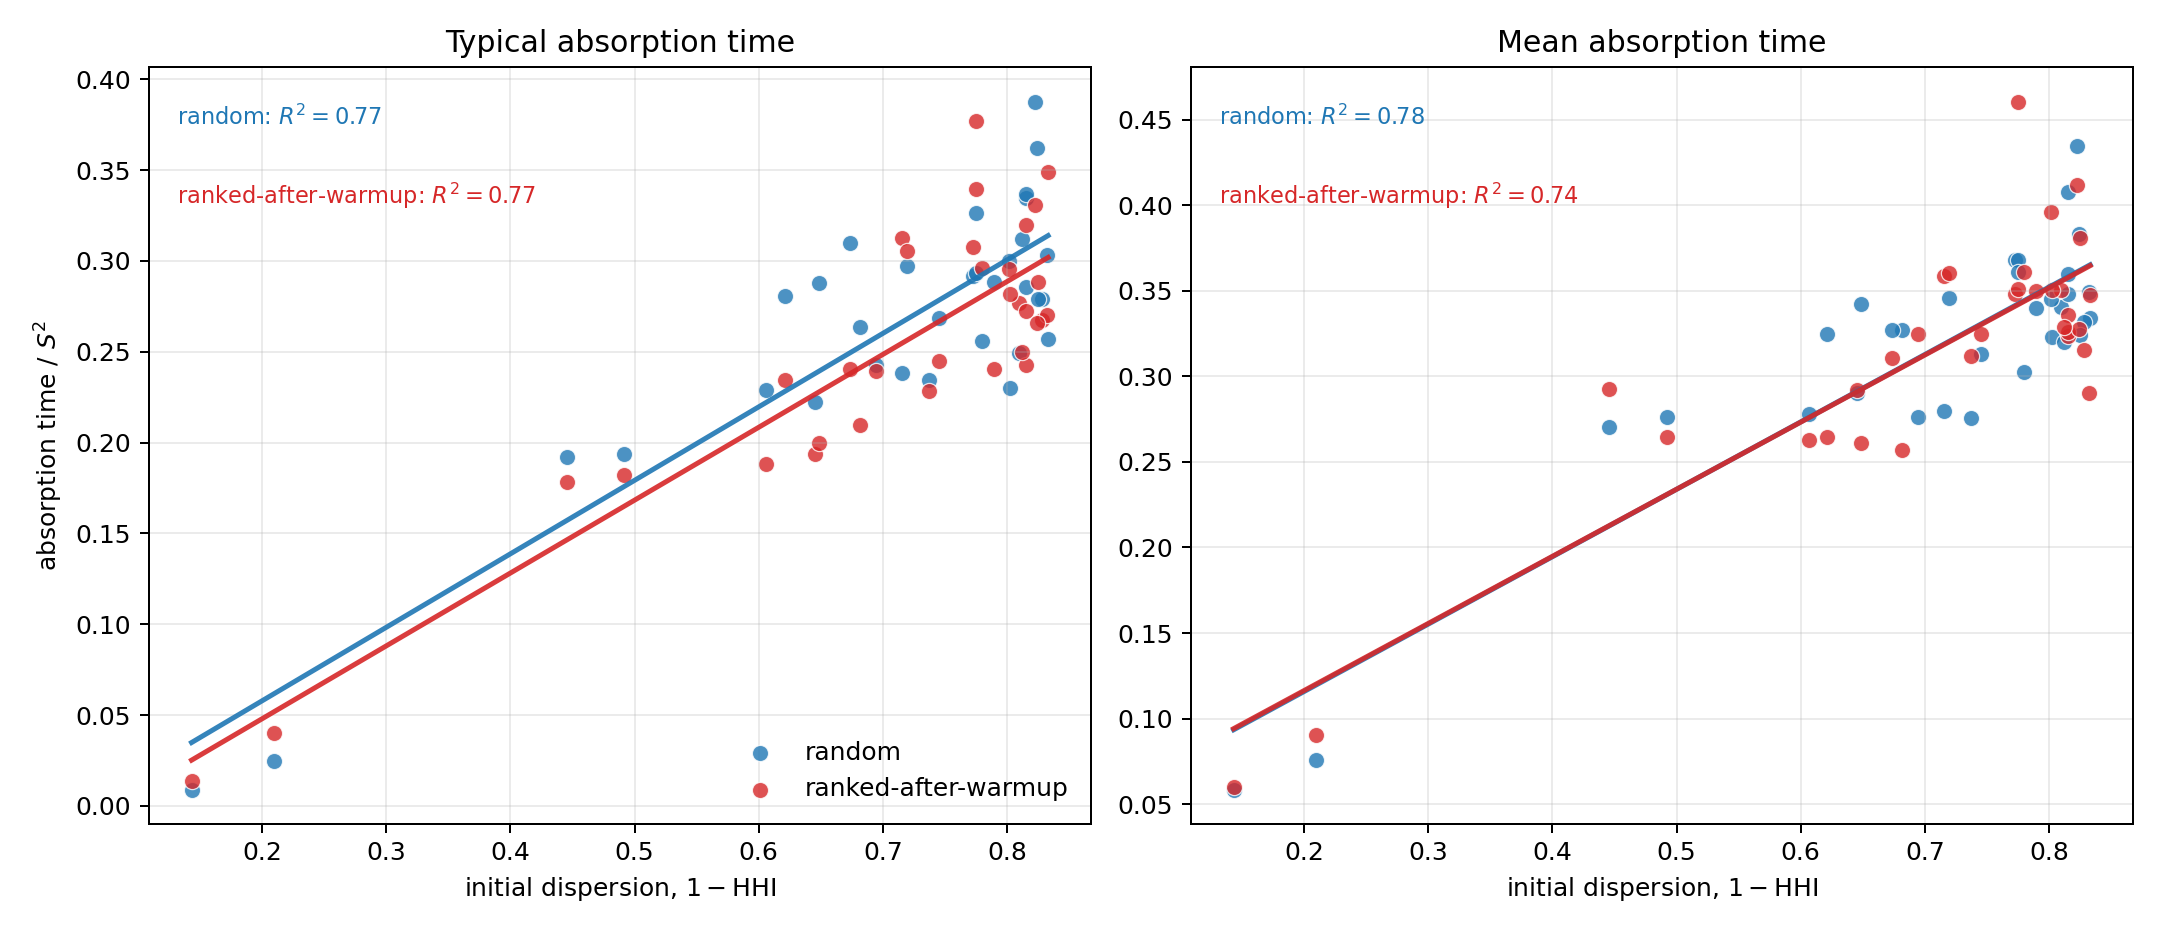
\includegraphics[width=\textwidth]{figures/concentration_vs_time.png}
  \caption{Initial wealth dispersion predicts absorption time. Each point is one initial wealth vector. The response is normalized by $S^2$. The fitted lines show that $1-\mathrm{HHI}$ captures much of the variation in both median and mean absorption time.}
  \label{fig:concentration}
\end{figure}

\begin{table}[htbp]
  \centering
  \begin{tabular}{lrrrr}
\toprule
Strategy & Vectors & Slope & Intercept & $R^2$ \\
\midrule
Random & 33 & 0.405 & -0.023 & 0.771 \\
Ranked after warmup & 33 & 0.401 & -0.032 & 0.775 \\
\bottomrule
\end{tabular}

  \caption{Linear fit of normalized median absorption time on $1-\mathrm{HHI}$. The slope is positive for both strategies, and the fit is strong for a one-predictor model.}
  \label{tab:regression}
\end{table}

\subsection{The pairwise product gives the same story}

Figure~\ref{fig:pairwise} uses the pairwise wealth-product predictor
\[
  \sum_{i<j} A_iA_j.
\]
For fixed $S$, this is equivalent to $1-\mathrm{HHI}$ up to scale. Its interpretation is useful: it is the sum of all two-player ruin time scales present in the initial population.

\begin{figure}[htbp]
  \centering
  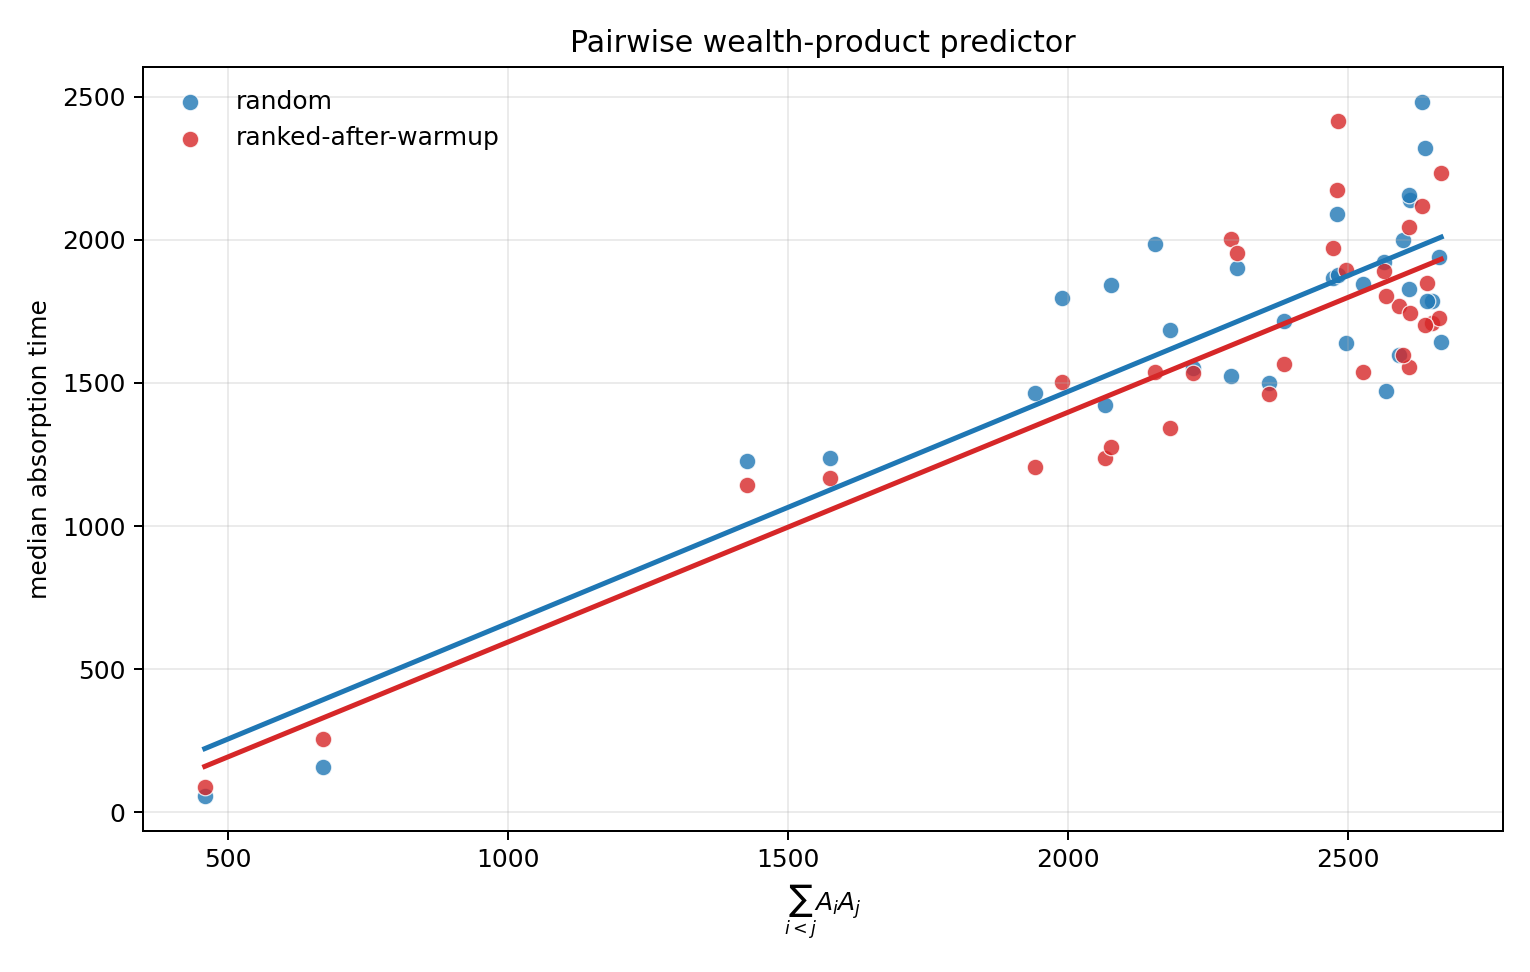
\includegraphics[width=0.86\textwidth]{figures/pairwise_product_vs_time.png}
  \caption{Median absorption time against the pairwise wealth-product sum. This is the most direct multi-player generalization of the two-player identity $\mathbb{E}[T]=A_1A_2$.}
  \label{fig:pairwise}
\end{figure}

\subsection{Distribution families}

Table~\ref{tab:families} aggregates by the distribution family used to generate the initial vectors. The family labels are not the theory; they are a way of spanning different concentration regimes. The more concentrated families tend to have smaller $1-\mathrm{HHI}$ and shorter normalized absorption times. The corresponding family bar plot is generated as \texttt{figures/family\_absorption\_bars.png}.

\begin{table}[htbp]
  \centering
  \begin{tabular}{lrrrr}
\toprule
Family & Vectors & Mean $1-\mathrm{HHI}$ & Random med. $T/S^2$ & Ranked med. $T/S^2$ \\
\midrule
Equal & 1 & 0.833 & 0.257 & 0.349 \\
Linear & 4 & 0.755 & 0.285 & 0.266 \\
Geometric & 4 & 0.781 & 0.265 & 0.291 \\
One Whale & 4 & 0.675 & 0.255 & 0.223 \\
Two Whales & 4 & 0.785 & 0.303 & 0.290 \\
Dirichlet & 16 & 0.655 & 0.249 & 0.228 \\
\bottomrule
\end{tabular}

  \caption{Distribution-family aggregates. Values are averaged over initial vectors within each family.}
  \label{tab:families}
\end{table}

Family effects are present, but the more important axis is concentration. Different families can land at similar $1-\mathrm{HHI}$ values and then have similar absorption times.

\section{Interpretation}

The results support a simple mechanism. Absorption is slow when there are many substantial cross-player wealth products. Equal or near-equal initial wealth creates many possible large contests, so the system wanders for a long time before a single stack captures the population. Concentrated initial wealth starts closer to monopoly and has fewer large opposing stacks, so absorption is faster.

The ranked-after-warmup policy does not overturn this relationship. It changes who plays whom, but the same initial-concentration predictor remains strong. In this first sweep, ranked pairing has a similar slope and explanatory power to random pairing. This suggests that initial wealth dispersion controls the dominant time scale, while strategy changes secondary features such as local trajectory shape, tail behavior, and perhaps constants in larger systems.

\section{Limitations}

This is an intentionally small-system experiment. We chose $N=6$ and $S=80$ so that simulations could run to true absorption. Larger systems can have very long absorption times. If a finite horizon $T_{\max}$ is imposed, unfinished runs should be treated as right-censored observations:
\[
  T > T_{\max},
\]
not as exact observations equal to $T_{\max}$.

For large systems, the right lens is survival analysis. The natural object becomes
\[
  \mathbb{P}(T>t),
\]
estimated by concentration bucket and strategy. The small-system absorption curves in this paper are therefore the clean no-censoring baseline.

\section{Conclusion and Future Work}

This first empirical paper establishes a plausible and useful regularity: for fixed $N$ and $S$, initial wealth dispersion predicts the time to absorption. The most natural predictor is
\[
  \sum_{i<j} A_iA_j
  =
  \frac{S^2}{2}(1-\mathrm{HHI}).
\]
In the present sweep, a one-variable linear model using $1-\mathrm{HHI}$ explains about 77\% of the variation in normalized median absorption time under both random pairing and ranked-after-warmup pairing.

The next steps are:
\begin{enumerate}
  \item Run the same initial vectors under additional strategic pairing policies.
  \item Scale the small-system sweep across $N$ and $S$ to check the $S^2$ normalization.
  \item Replace full absorption-time estimation by survival curves for large systems.
  \item Study whether Gini, max share, or entropy explain residual variation beyond $1-\mathrm{HHI}$.
  \item Connect windowed Hurst estimates of trajectories to absorption-time regimes.
\end{enumerate}

The working thesis is that fair play determines who wins in expectation, but initial concentration determines how long the system remains plural.

\end{document}
